\section{Overview}

Performance of the Earth Networks Total Lightning Network (ENTLN) is evaluated with respect to the TRMM Lightning Imaging Sensor (LIS).
ENTLN lightning strokes are matched to LIS lightning flashes from 2011 -- 2013 over the continental United States and within the 35$^\circ$ orbital inclination of LIS.
ENTLN matched $1.4\times10^5$ of the $2.1\times10^5$ LIS flashes with a total of $4.8\times10^5$ strokes, giving an average multiplicity of 3.5 and 66\% detection efficiency of all flashes.
Over the course of the evaluation period the average daily detection efficiency was $69\pm14$\%.
The median timing offset from the first ENTLN stroke was 2.4~ms (LIS leading) with a sharp peak at -1.9~ms; the median distance offset was 7.0~km from the flash centroid.
The sharp peak at -1.9~ms is likely caused by inherent differences in the detection techniques: LIS observes light emitted from the tops of the clouds and ENTLN measure the radio signals from the return stroke.
%During this period ENTLN detected a total of $3.1\times10^8$ strokes within the observation region, additional capabilities of the network such as peak current estimates and stroke type discrimination were not directly examined.

The performance of LIS relative to ENTLN is also evaluated by finding all ENTLN strokes located within the LIS field of view.
LIS matched 68\% of the $7.1\times10^5$ ENTLN strokes to observed flashes in the LIS field of view.
The $70\pm12$\% daily average LIS detection efficiency of ENTLN strokes demonstrates that neither system detects every flash or stroke located by the other.
Assuming a 3.5 multiplicity of ENTLN unmatched strokes, LIS did not detect $6.6\times10^4$ flashes, or 31\% of all flashes.
The ENTLN-LIS matched strokes were $20.3\pm0.6$\% cloud to ground and unmatched strokes were $21.8\pm0.8$\% cloud to ground.
There is a marginal difference in the lightning populations sampled by both systems;  LIS is slightly biased towards cloud flashes.

There is a growing importance, both scientifically and operationally, of ground based lightning detection networks.
Lightning detection networks are being used in a larger gamut of research areas including: terrestrial gamma ray flashes \citep{Dwyer2012, Gjesteland2011, Connaughton2010}, lightning climatology \citep{Virts2013, Virts2011a, Burgesser2012}, ionospheric disturbances and probing \citep{Jacobson2010, Singh2011}, transient luminous events \citep{Soula2011}, global electric circuit  \citep{Holzworth2005}, and whistler observation \citep{Collier2010, Collier2011a, Burkholder2013}.
This is in conjunction with the extended usage of lightning networks operationally in weather prediction and tracking \citep{Fierro2012, Pan2010, Thomas2010d}, volcano monitoring \citep{Doughton2010}, and hazard estimation \citep{Altaratz2010}.
With growing usage it is necessary to understand the capabilities and efficiencies of the various available lightning networks.

Ground based total lightning networks distinguish themselves from other ground based networks and satellites by detecting and identifying in-cloud (IC) discharges as well as cloud to ground (CG) strokes.
Lightning type is critical in understanding thunderstorm dynamics \citep{Williams1989}, with real time monitoring of sudden increases of IC activity able to predict severe weather events \citep{Rudlosky2013, Darden2010, Metzger2013, Schultz2009, Schultz2011}.
The higher frequencies of total lightning networks are also useful for researching narrow bipolar events \citep{Suszcynsky2003} and large scale lightning behavior \citep{Hutchins2013}.
Lightning mapping arrays are able to locally detect, locate, and distinguish IC activity, however total lightning networks have the advantage of much larger spatial coverage.

To evaluate the ENTLN performance it is compared against the Lightning Imaging Sensor (LIS) onboard the Tropical Rainfall Measurement Mission (TRMM) satellite orbiting at a 35$^\circ$ inclination \citep{Christian1999}.
LIS is used as a reference system as the sensor performance has not changed over time and it is uses a different detection method (optical) than ground networks. 
The LIS data are available at several processed levels, the 2011 -- 2013 flash level data is used for this comparison.
The comparison with LIS is made over North America and within the inclination of LIS, the area covered is shown in Figure~\ref{entln_lis:fig:density}.
In this region LIS located $2.1\times10^5$ flashes, with the distribution shown in Figure~\ref{entln_lis:fig:density}a, and ENTLN located $3.1\times10^8$ strokes shown in Figure~\ref{entln_lis:fig:density}b.
ENTLN detected $1.4\times10^5$ strokes within the field of view of LIS.

\begin{figure}[t]
   \centering
   \noindent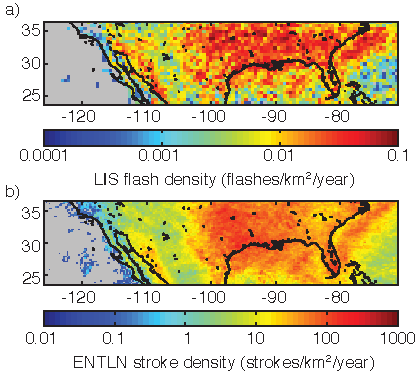
\includegraphics[width=19pc,angle=0]{entln_lis/Figures/density.pdf}
   \caption{a) LIS flash density at 0.5$^\circ$ grid spacing for fully viewed granules and
   		b) ENTLN stroke density at 0.25$^\circ$ grid spacing for 2011 -- May 2013.
   		Densities normalized to counts/km$^2$/year, grid points with less than 30 counts are shown in gray.}
   \label{entln_lis:fig:density}
\end{figure}

Utilizing lightning networks requires a thorough understanding of what the networks detect and their limitations.
Examining detection efficiencies is one method to characterize the performance of networks, however such measures need to be used carefully as they often necessitate the assumption that the reference system is uniform, constant, and complete.
Using the LIS instrument allows for a robust and standard analysis of the ENTLN efficiency and accuracy.

\section{Performance}

\subsection{Matching}

ENTLN strokes are matched to LIS flashes when the ENTLN stroke is within a $\pm0.5^\circ$ box around the flash centroid and within $\pm10$~ms of the flash duration.
If multiple strokes are matched to a single LIS flash the timing and location of the stroke closest in time to the start of the flash is used as the best match.
For the case of multiple flashes matched to a single stroke only the flash closest in time to the stroke is matched.
Matches between ENTLN-LIS had 30\% of LIS flashes matched to a single ENTLN stroke, with an overall mean multiplicity of 3.5.
Days with less than 30 total LIS flashes over North America are not used in this evaluation.

%% Add in a viewpoint granule figure?

Evaluation of the effectiveness of LIS at observing ENTLN strokes utilizes the viewpoint granule data available with the flash level data.
The viewpoint granules give the start and end times of LIS observation for $0.5^\circ \times 0.5^\circ$ bins.
Full coverage for a given viewpoint granule is determined by the start and end times of the adjacent corner granules.
When LIS has at least partial coverage of the four corner viewpoint granules the center viewpoint granule is guaranteed to be in full view of the sensor.
The latest start time and earliest end time of the adjacent corner granules determines the time when the viewpoint granule is in full view of LIS.
Only ENTLN strokes and LIS flashes within viewpoint granules with full LIS coverage are used in this evaluation.
This restriction reduces the total number of LIS flashes by 30\% from $3.0 \times 10^5$ to $2.1 \times 10^5$ flashes.
This restriction on strokes and flashes ensures that all ENTLN strokes are within full view of LIS, removing edge and partial view cases.

An example of a single LIS overpass full coverage field of view, determined by the viewpoint granules, is shown in Figure~\ref{entln_lis:fig:overpass}.
This overpass occurred on 2012 April 21 from 15:20 -- 15:31 UTC.
Within the field of view LIS observed 220 flashes, of which ENTLN matched 66\%, shown in Figure~\ref{entln_lis:fig:overpass}a.
ENTLN strokes are considered within the field of view of LIS if they occur within the bounds of the viewpoint granule and between the start and end time of full LIS coverage.
In the pass shown in Figure~\ref{entln_lis:fig:overpass}b ENTLN detected 773 strokes, where 67\% were matched to LIS flashes.
In both cases the missed events are shown as red crosses.

\begin{figure}[t]
   \centering
   \noindent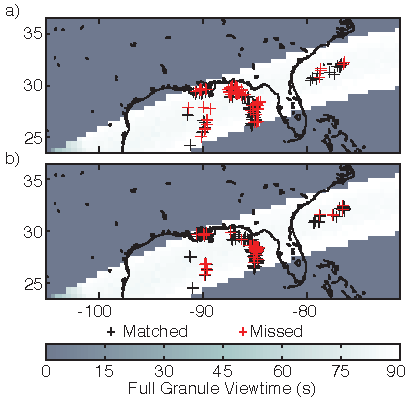
\includegraphics[width=19pc,angle=0]{entln_lis/Figures/overpass.pdf}
   \caption{LIS observation area for 2012 April 21 from 15:20 -- 15:31 UTC (day), seconds within full view of LIS shown in grayscale.
      		a) shows the LIS flashes matched by ENTLN (black crosses) during the overpass, red crosses are LIS flashes missed by ENTLN.
		b) shows the ENTLN strokes matched by LIS (black crosses) during the overpass, red crosses are ENTLN strokes missed by LIS.
		}
   \label{entln_lis:fig:overpass}
\end{figure}

\subsection{Accuracy}

System accuracy is measured by the timing and spatial offset between the lightning locations.
The timing offset ($t_{LIS} - t_{ENTLN}$), Figure~\ref{entln_lis:fig:accuracy}a, is sharply peaked at -1.9~ms, with ENTLN occurring before the LIS flash time; the median timing offset is 2.4~ms.
The LIS flash time is the time of the first LIS event in the flash group; 42\% of ENTLN strokes occurring 0 -- 4~ms before the start of the LIS flash, the remaining strokes correspond to other discharges of the flash.

\begin{figure}[t]
   \centering
   \noindent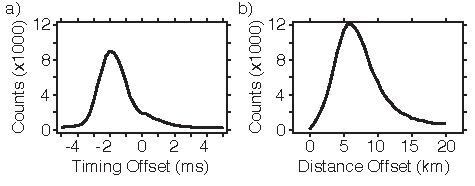
\includegraphics[width=19pc,angle=0]{entln_lis/Figures/accuracy.pdf}
   \caption{a) ENTLN-LIS timing offset ($t_{LIS} - t_{ENTLN}$) for the first matched stroke and
   		b) ENTLN stroke to LIS flash centroid distance for the first matched stroke.
   		Bin spacing set at (a) 0.25~ms and (b) 0.5~km.}
   \label{entln_lis:fig:accuracy}
\end{figure}

The median distance offset from the flash centroid is 7.0~km, as seen Figure~\ref{entln_lis:fig:accuracy}b, slightly above the LIS spatial resolution of 3 -- 6~km \citep{Christian1999}.
The location offset can be given in either kilometers from the flash centroid or in units of the estimated flash radius, where the radius is calculated by considering the given LIS flash area as a circle.
Using the flash radius for distance results in a median offset of 0.80 flash radii, 65\% of the strokes are located within the visible extent of the flash.
The exact location accuracy of ENTLN cannot be determined with LIS due to the spatial accuracy of the LIS pixels.

\subsection{Detection efficiency}

During the 2011 -- 2013 evaluation period the average daily detection efficiency of LIS flashes by ENTLN was 69\% $\pm$ 14\%.
The detection efficiency was marginally higher during the day at 72 $\pm$ 14\% and lower during the night at 65 $\pm$ 16\%.
The ENTLN decrease at night likely stems from the increased detection efficiency of LIS at observing lightning against a non-sunlit ground.
The spatial distribution of detection efficiency is shown in Figure~\ref{entln_lis:fig:map}a, with the daily variability shown in Figure~\ref{entln_lis:fig:de}a.
The spatially averaged detection efficiency is $61 \pm 16$\%, due to the uneven distribution of ENTLN stations with fewer stations in the West.
ENTLN detected 66\% of the $2.1\times10^5$ LIS flashes, within those flashes ENTLN detected $7.4\times10^5$ strokes ($<0.15$\% of total ENTLN strokes).
ENTLN has a spike of low detection efficiency in mid-June 2012 that is reflected in the LIS detection efficiency, this temporary decrease is likely due to a short-term issue with the network.

\begin{figure}[t]
   \centering
   \noindent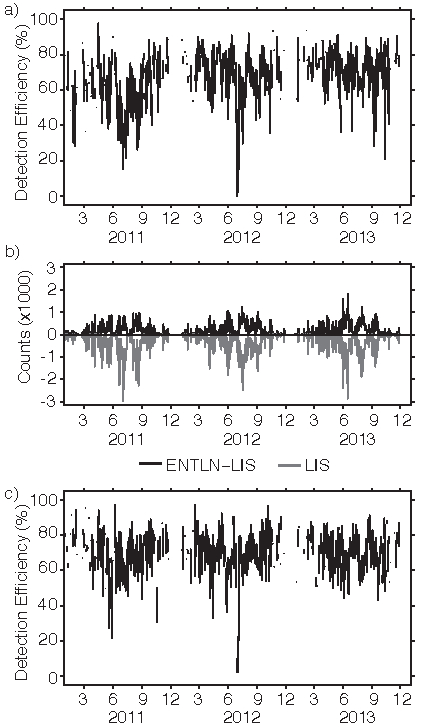
\includegraphics[width=19pc,angle=0]{entln_lis/Figures/de.pdf}
   \caption{a) ENTLN-LIS daily detection efficiency,
   		b) ENTLN-LIS total matches (black) and total LIS flashes (gray),
		c) LIS daily detection efficiency of ENTLN strokes.
		Gaps indicate days with less than 30 LIS flashes.
		}
   \label{entln_lis:fig:de}
\end{figure}

Within the LIS field of view ENTLN detected $7.1\times10^5$ strokes, of these strokes $4.8\times10^5$ were matched to LIS flashes for an overall LIS detection efficiency of ENTLN strokes of 68\%.
The spatial distribution of LIS detection efficiency of ENTLN strokes is shown in Figure~\ref{entln_lis:fig:map}b and the daily detection efficiency is shown in Figure~\ref{entln_lis:fig:de}c.
The average spatial variability of LIS is $67 \pm 13$\%, with an average daily detection efficiency of $70 \pm 12$\%.
Assuming the same multiplicity of 3.5 for the unmatched ENTLN strokes LIS missed $6.6\times10^4$, or 31\%, of all flashes.
To test for the possibility that the strokes not detected by LIS were improperly located, the waveforms for a random subset for ENTLN strokes were examined and the locations were found to be correct.

\begin{figure}[t]
   \centering
   \noindent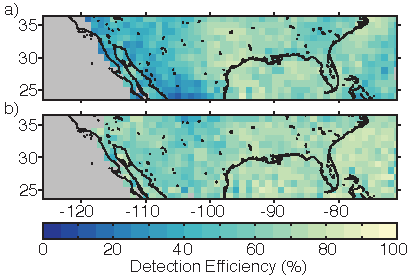
\includegraphics[width=19pc,angle=0]{entln_lis/Figures/map.pdf}
   \caption{a) Spatial distribution of ENTLN detection efficiency of LIS flashes and
   		b) LIS detection efficiency of ENTLN strokes.
   		Gray indicates $1^\circ \times 1^\circ$ bins with fewer than 30 LIS flashes.
		}
   \label{entln_lis:fig:map}
\end{figure}

Over land the highest ENTLN detection efficiency can be seen to occur in the Great Plains, Florida, and Texas.
There is decreased detection efficiency over both the Rocky and Appalachian Mountains, likely caused by the lower sensor density in these regions.
While the mountain regions show lower detection efficiency with lower sensor density, there is a higher and more uniform detection efficiency within 450~km off the coasts.
The increased detection efficiency off of the coasts is a combined effect of fewer and stronger lightning strokes \citep{Hutchins2013, Rudlosky2010}.
LIS has a more uniform detection efficiency than ENTLN, as is expected from the imaging system.

On a daily scale the ENTLN-LIS detection efficiency, seen in Figure~\ref{entln_lis:fig:de}a, is fairly high through this time period, with brief periods of decreased performance.
The average daily detection efficiency is 69 $\pm$ 15\% with a $5^\text{th}$ to $95^\text{th}$ percentile range of 48\% -- 87\%.
Some of the larger decreases in detection efficiency match with the increased LIS flash counts in Figure~\ref{entln_lis:fig:de}b, such as early April 2012, late May 2012, and mid-July 2012.
On days with low LIS flash counts, $<40^\text{th}$ percentile, ENTLN detects $71\pm16$\% of flashes; while on days with high LIS flash counts, $>70^\text{th}$ percentile, ENTLN detects $65\pm10$\% of flashes.
During these times of increased lightning activity the ENTLN would need to raise the data compression threshold; causing it to miss weaker strokes that are still detected by LIS, resulting in the suppressed detection efficiency.

\subsection{Observation bias}

Two populations of ENTLN strokes are found with the comparison to LIS: the strokes matched to LIS flashes and the strokes that are unmatched.
Characteristics of these populations should show any bias of the flashes that are observed by LIS.
As ENTLN is a total lightning network it has the capability to detect and distinguish between CG and IC strokes.

To get a statistically robust measure of the percentage of cloud to ground strokes observed by LIS the matched LIS-ENTLN stroke data was randomly subdivided into 100 subsets of approximately $4.8\times10^3$ matched strokes.
Averaging these subsamples results in the statistically robust measure of the matched stroke CG percentage.
The populations of matched and unmatched LIS-ENTLN strokes are very similar, matched strokes are $20.3\pm0.6$\% CG and unmatched strokes are $21.8\pm0.8$\% CG.
The small difference between the population shows that there is only marginal detection efficiency bias between lightning observed by LIS and ENTLN, with LIS slightly biased towards cloud flashes.

\section{Conclusion}

Characterizing the ENTLN, and other ground based networks, relative to a uniform detection system is critical in enabling the application of these networks in scientific and operational uses.
The Earth Networks Total Lightning Network was compared to the TRMM/LIS instrument on a stroke to flash matching level.
An average daily detection efficiency of $69\pm 14$\% was found for the continental United States for January 2012 -- May 2013 for $2.1 \times 10^5$ LIS flashes.
The relative location accuracy with respect to the flash centroid is 7.0~km and a timing offset to the start of the flash of 2.3~ms.
Within the LIS field of view ENTLN located $7.1\times 10^5$ strokes and $3.1\times10^8$ strokes within the entire evaluation region.
Of those located ENTLN strokes LIS had a $70 \pm 12$\% detection efficiency, resulting in an estimated $6.6 \times 10^4$ flashes (31\% of total flashes) not detected by LIS.
Long range ground networks have the advantage of continuous real-time coverage of their encompassed region, resulting in more strokes detected along with capabilities such as stroke type discrimination and peak current.

\subsection*{Acknowledgments}

The LIS flash data were obtained from NASA's Global Hydrology Resource Center (http://thunder.msfc.nasa.gov).
